\chapter{Methodes Agiles}
TODO : déroulement d'un semaine "agile"
Méthode Agile : eXtreme Programming  (XP)
Les méthodes Agiles et l'eXtreme Programming sont un ensemble de bonne pratiques dédiées à la production logicielle. Elles ont comme philosophie accepter le changement plutôt que de le supporter. L'eXtreme Programming (XP) pr\^one les cycles de développement courts (1 à 2 semaines). Un Client XP\footnote{Client sur site interne} permet d'avoir des retours rapides et de s'assurer que les exigences fonctionnelles soient bien comprises et implémentées.

L'eXtreme Programming repose sur cinq valeurs
\begin{itemize}
\item{La communication}
\item{La simplicité}
\item{Le feedback}
\item{Le courage}
\item{Le respect}
\end{itemize}
\section{Itération}
L'équipe organise son travail sous forme d'itération, chaque itération traite un nombre de fonctionnalités limité quantifié sous forme de points de vélocité. Une itération est planifiée lors de la rétrospective de l'itération précédente. Un itération compte un certain nombre de points de vélocité qui est en fait un objectif à atteindre par l'équipe de développement. La durée d'une itération est en général inférieure à 2 semaines. A la fin d'une itération le produit est livré.
\begin{figure}[!h]
\centering
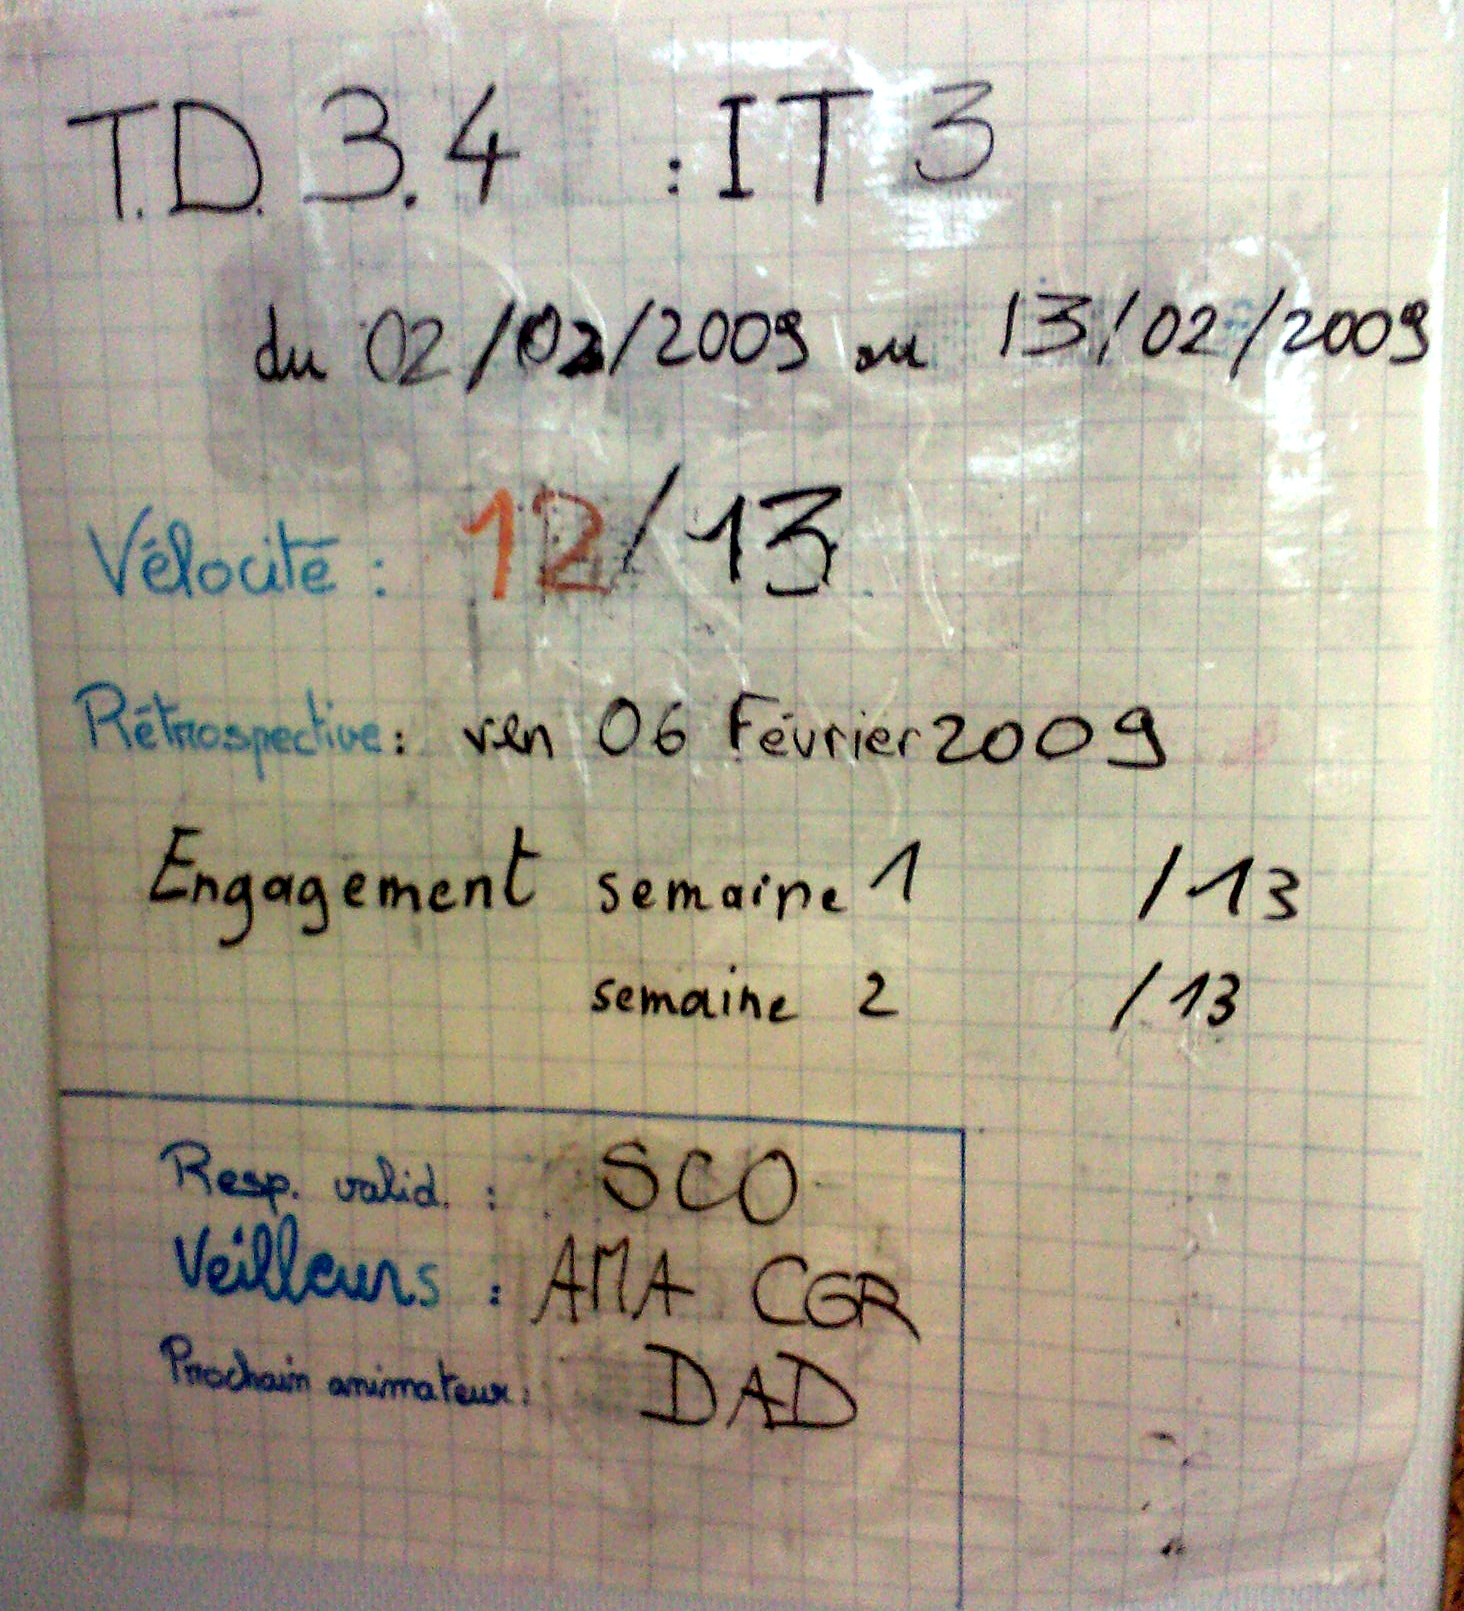
\includegraphics[scale=0.10]{Illustrations/SP_A0182.jpg}
\caption{Iteration}
\label{fig:Iteration}
\end{figure}

\section{Rétrospective}
Lors d'une rétrospective,  les membres de l'équipe de R\& D se réunissent pour parler de la précédente itération et pour planifier celle à venir. La réunion commence par un « check in » pendant lequel une question est posée (par exemple « Comment voyez vous Test Designer dans un an?).Un point sur des statistiques (métriques) telles que le nombre de lignes de code, le nombre de tests unitaires ou encore la vélocité atteinte par rapport aux objectifs est fait. Le point est ensuite porté sur les fonctionnalités qui ont été réalisées ou non lors de l'itération. La réunion se continue par les discussions diverses, chacun peut discuter de diverses choses : apparition de problèmes, amélioration du fonctionnement de l'équipe. La réunion se termine enfin par l'annonce de la prochaine vélocité et l'attribution des responsabilités pour l'itération qui vient. En effet chaque itération a des responsables différents (animateur de la rétrospective, validation, veilleur ...)
\section{Fiches}
Des fiches correspondent aux différentes t\^aches à effectuer dans le cadre d'une itération. Elles peuvent \^etre de type différent : valeur client (couleur blanche), T\^ache technique (couleur verte), Point technique (couleur bleue), Anomalie (couleur rouge), Amélioration de process (couleur jaune). Les couleurs des fiches permettent à l'équipe d'identifier au premier coup d'oeil le travail à réaliser et l'urgence. Si le tableau comporte beaucoup de fiches rouges, elles seront à traiter en priorité car ce sont des bugs. Les fiches possèdent des points qui correspondent à la quantité de travail à effectuer (en demie-journée par bin\^ome) sur la t\^ache. Si la fiche est trop importante elle peut être redécoupées en fiches plus petites.

%\caption{Tux, le pingouin}
%\label{Tux}
%
%Ensuite, on s'en sert comme d'habitude (noter l'utilisation du tilde -- espace insécable -- pour garder les numéros près des mots qui les introduisent) :
%
%Dans le tableau~\ref{Tux}, page~\pageref{Tux}, nous lisons...

\begin{figure}[!h]
\centering
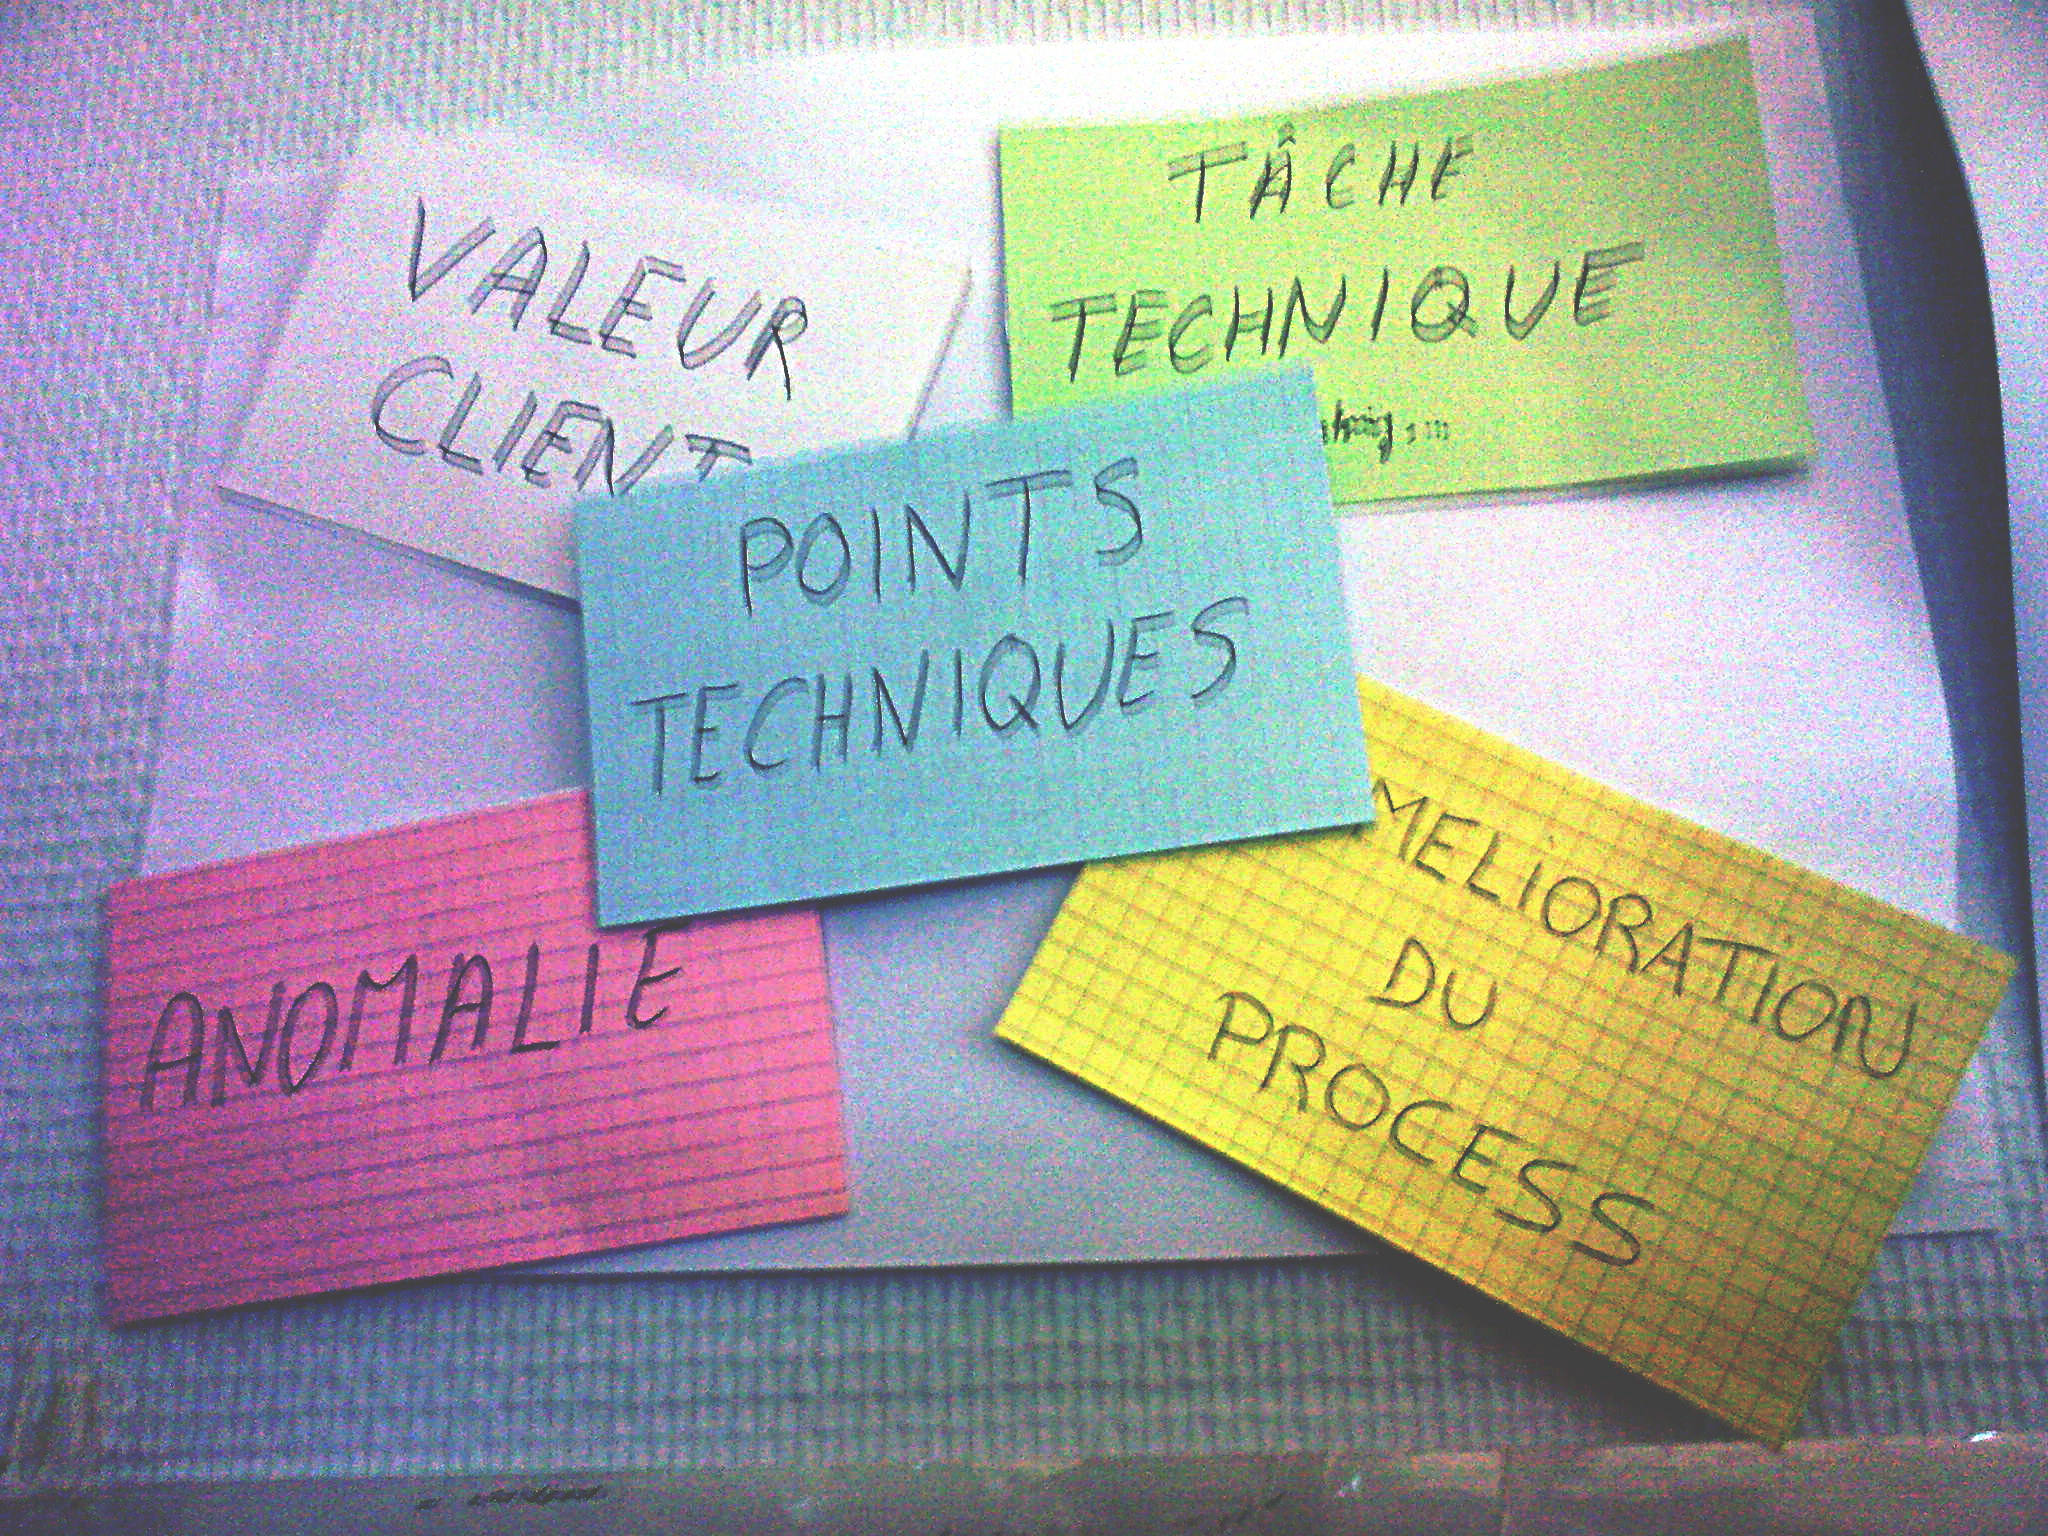
\includegraphics[scale=0.10]{Illustrations/SP_A0185.jpg}
\caption{Fiches}
\label{fig:Fiches}
\end{figure}
\begin{figure}[!h]
\centering
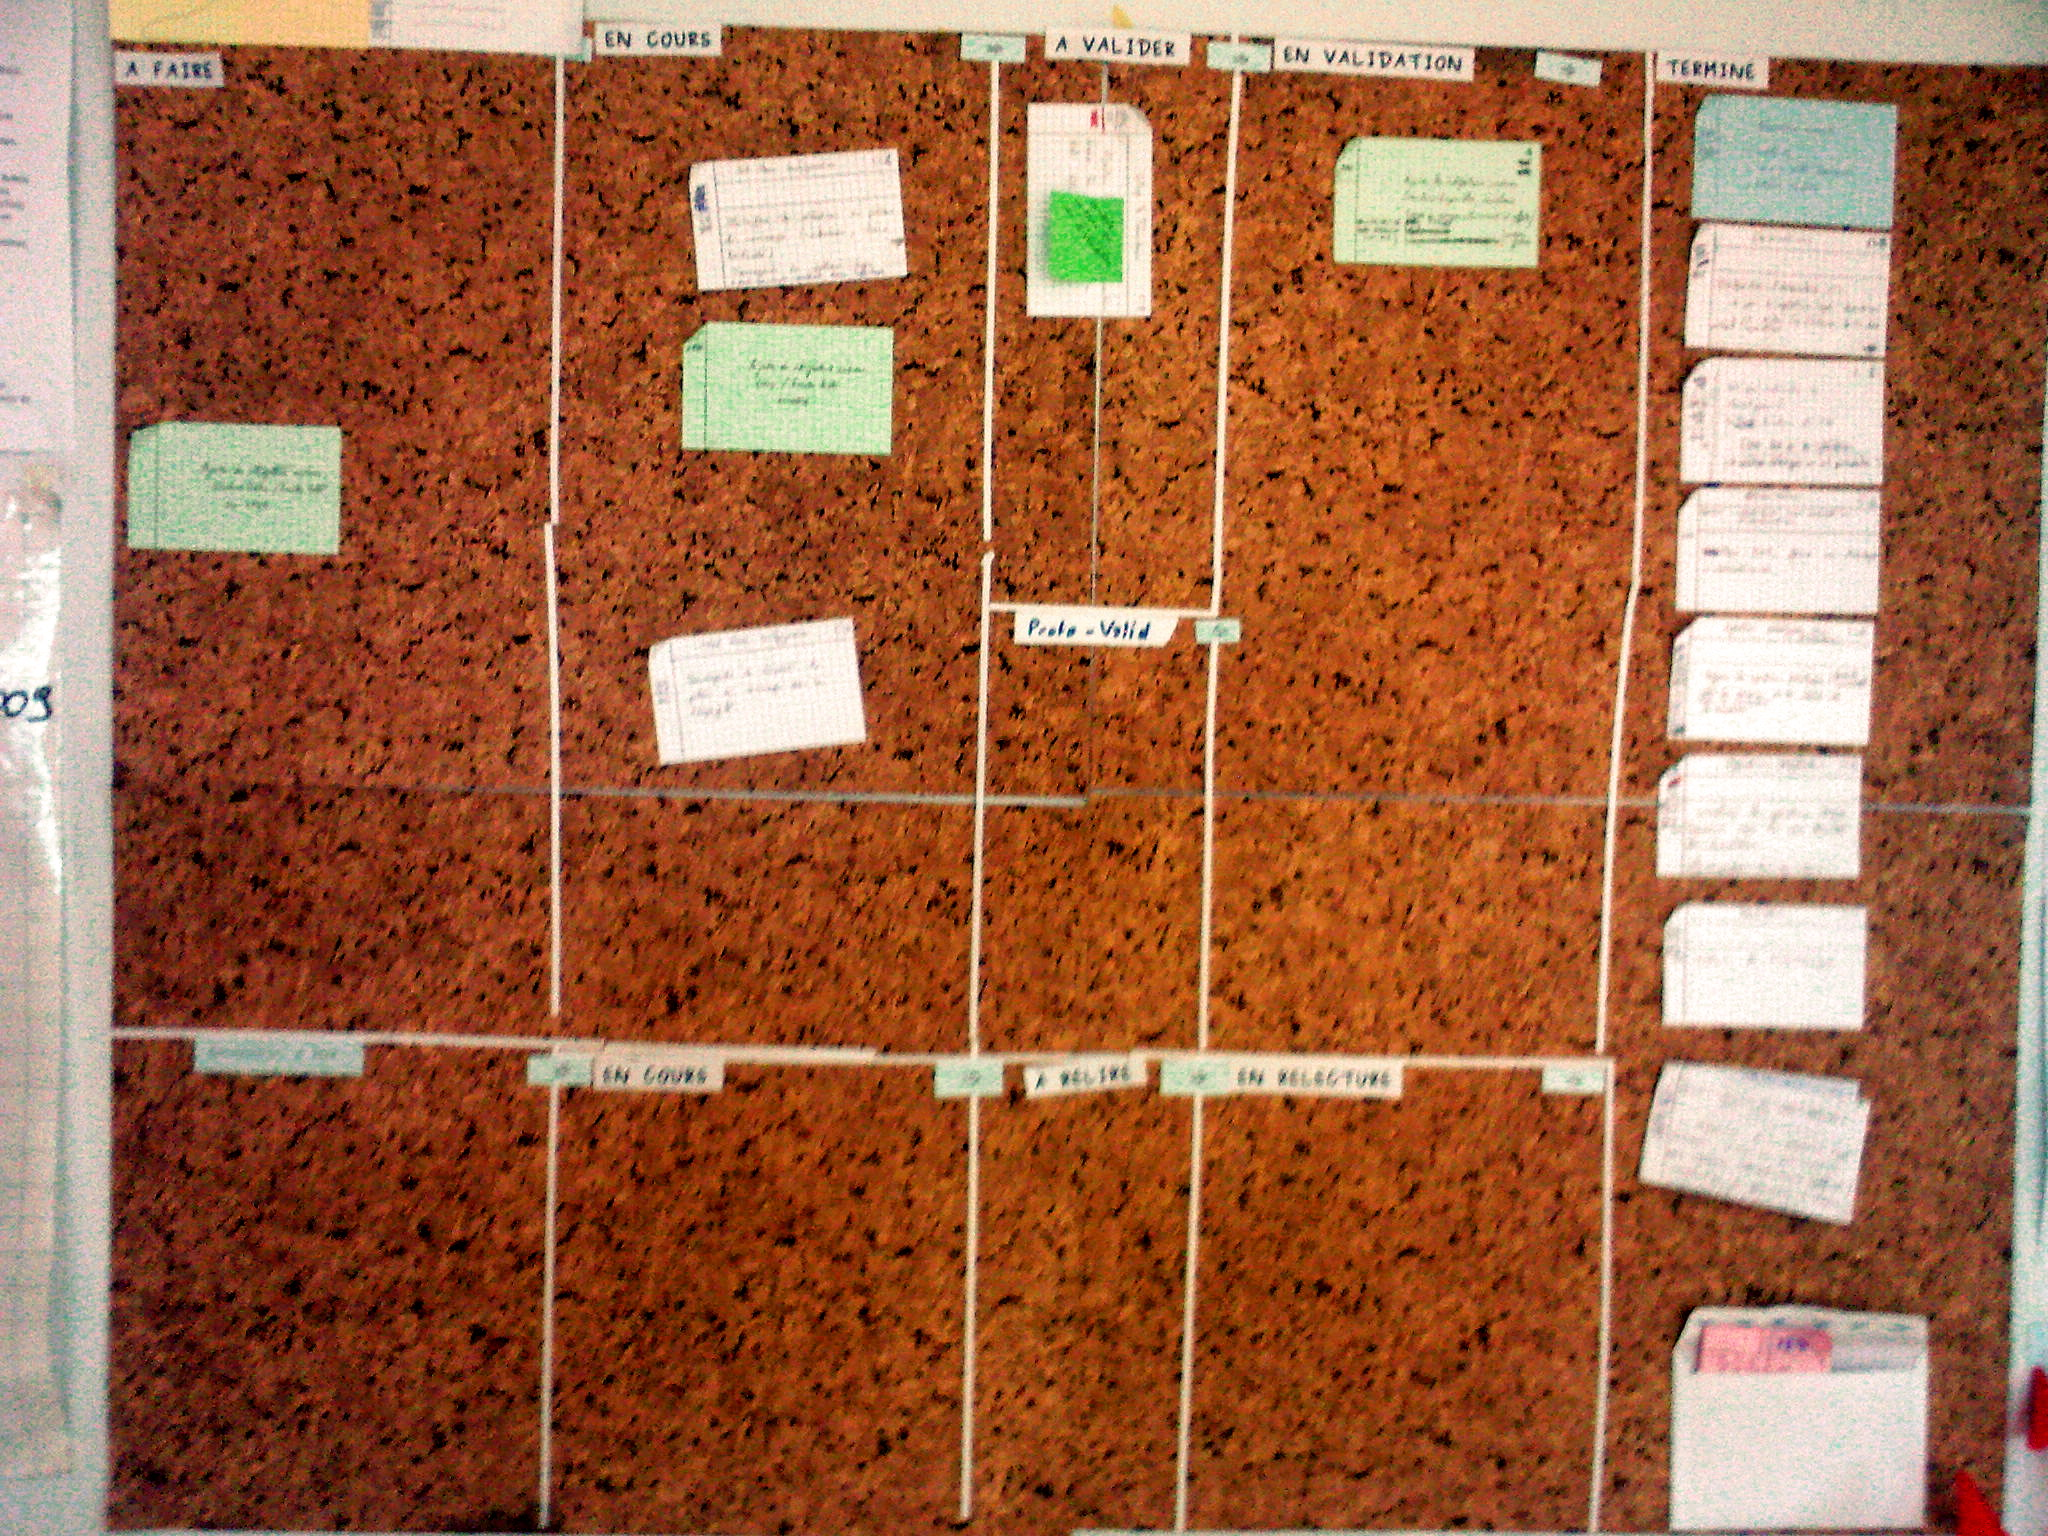
\includegraphics[scale=0.10]{Illustrations/SP_A0183.jpg}
\caption{Tableau d'avancement des fiches}
\label{fig:Tableau d'avancement des fiches}
\end{figure}
\section{Travail en binômes (pair programming)}
Une grand partie du travail dans l'équipe est réalisée en binôme. Les binômes changent très souvent. Les avantages du travail en binôme sont multiples. Contrairement à la programmation individuelle les binômes permettent de diffuser plus rapidement le savoir acquis lors du développement et seront plus à même à partager leur connaissances (effet boule de neige). De plus des études montrent que le travail par paires donne généralement un code de meilleure qualité, une meilleure capture des bugs. La communication et la motivation dans l'équipe sont également améliorées par cette méthode.
\begin{figure}[!h]
\centering
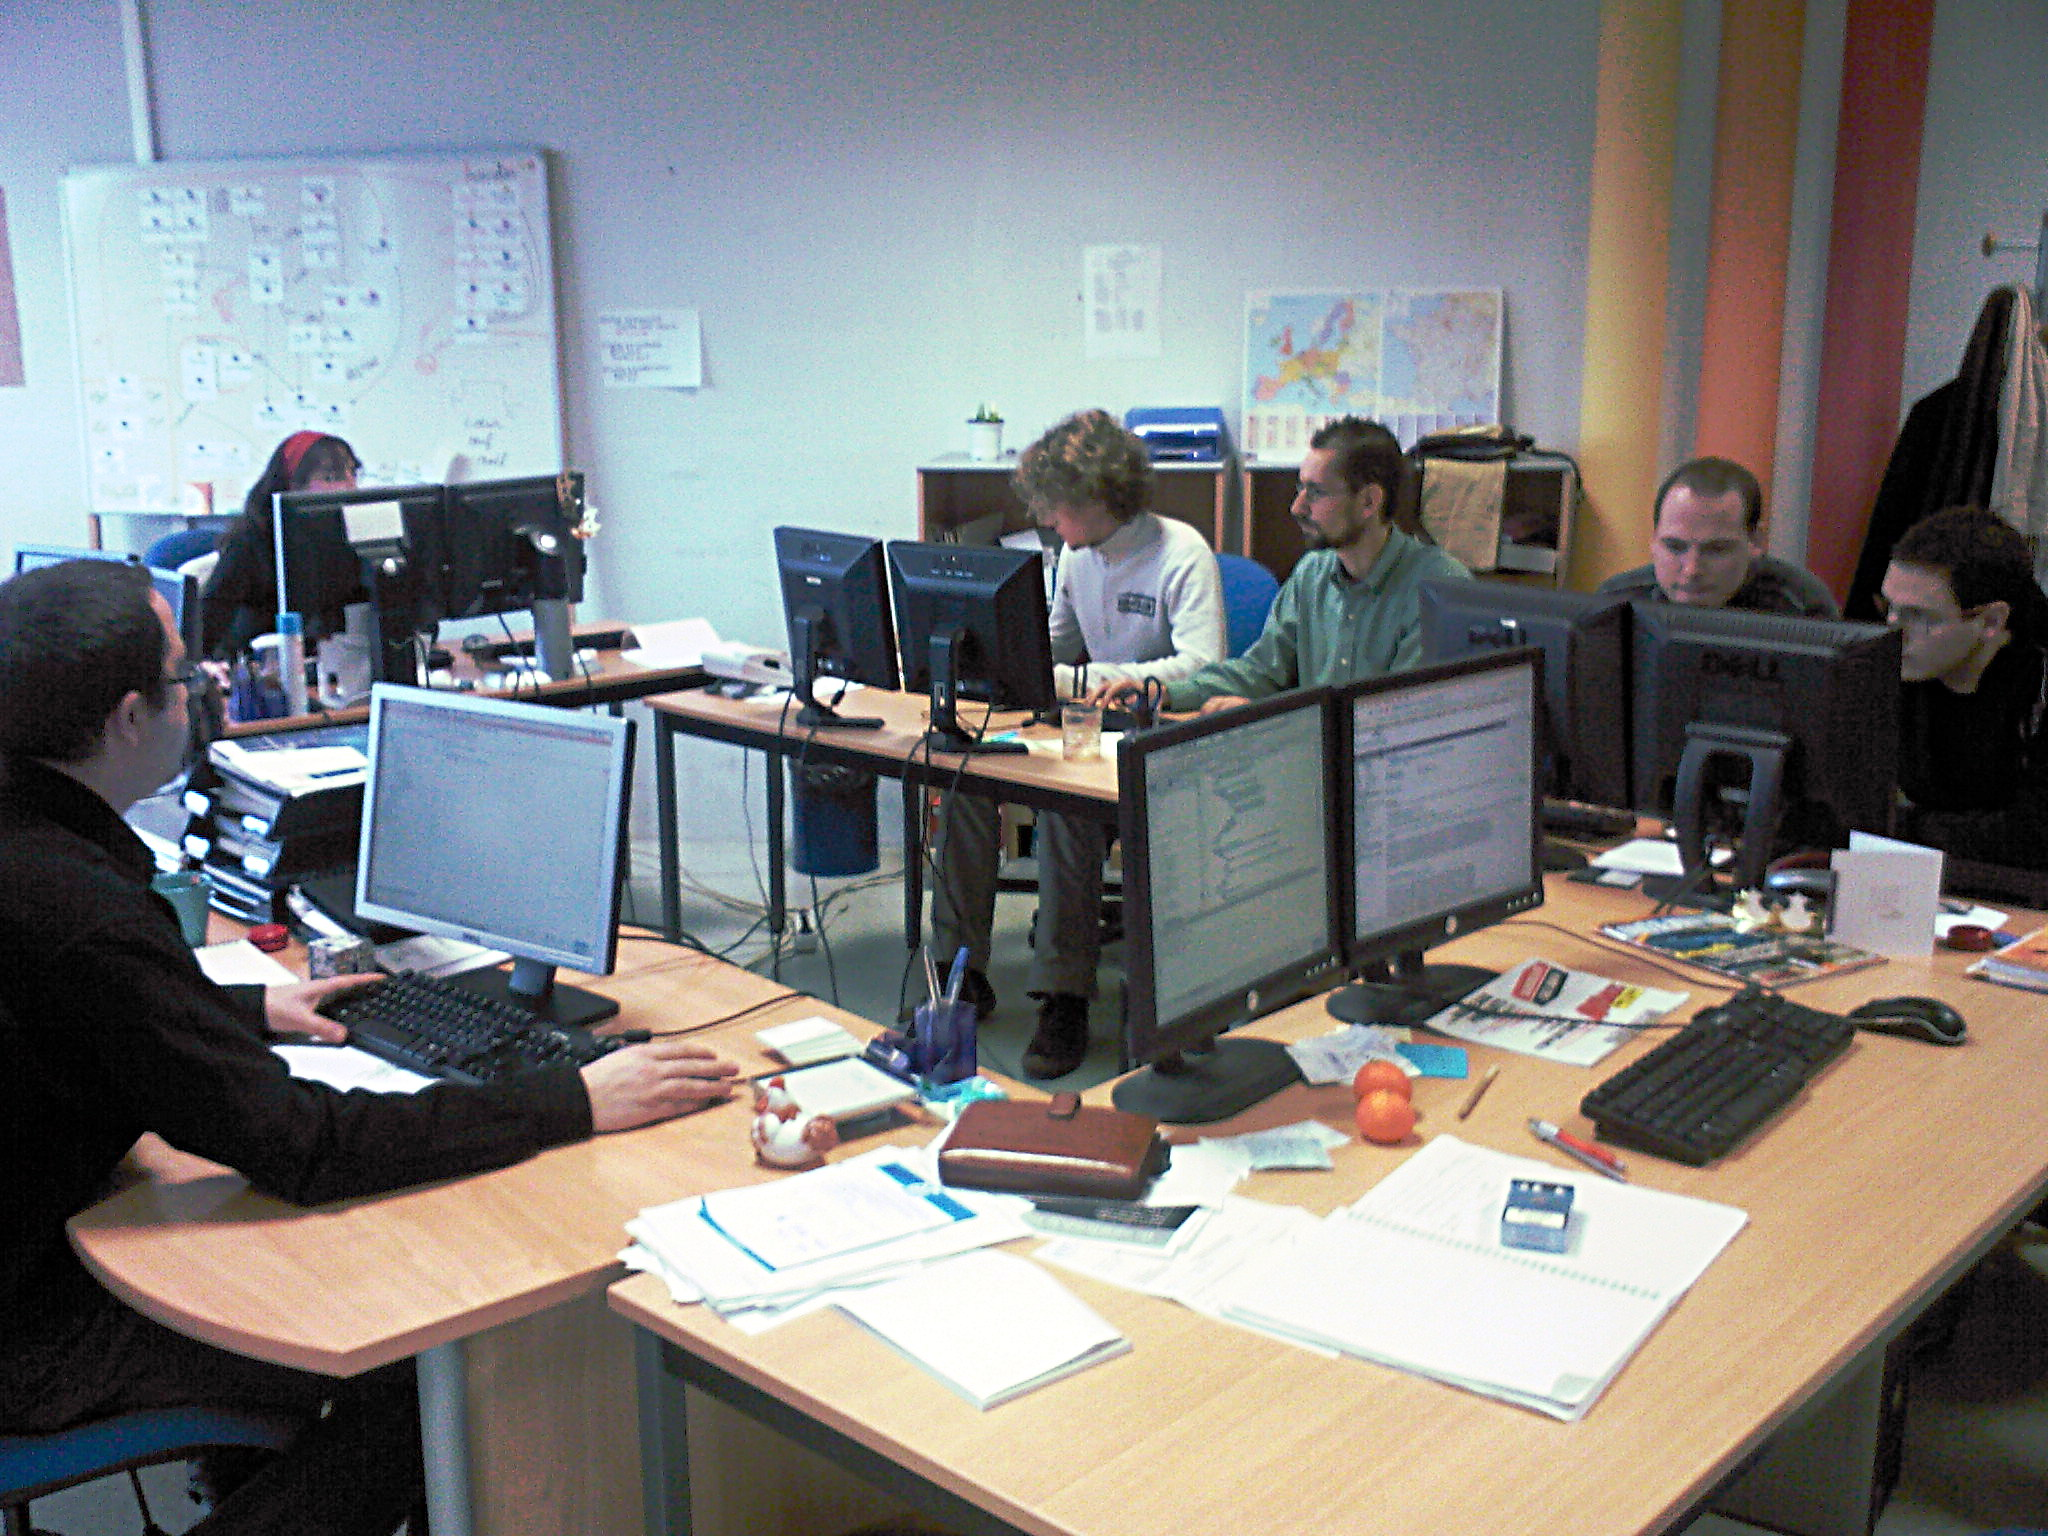
\includegraphics[scale=0.15]{Illustrations/SP_A0188.jpg}
\caption{Pair programming}
\label{fig:Pair programming}
\end{figure}
\section{Validation}
La validation joue un rôle important lors de l'intégration continue. Elle ne peut être réalisée que par des personnes qui n'ont pas participé au développement de la fonctionnalité. Cela permet d'avoir une idée plus objective des manipulations à effectuer pour tester la fonctionnalité. La validation es supervisée par le Client XP.


\section{Semaine type}
La semaine Agile 
\subsection{Morning meeting}
Les membre de l'équipe se réunissent juste avant la pause déjeuner pour parler de ce qu'ils ont fait la matinée afin d'informer toute l'équipe de l'avancée de leur engagement ainsi que des problèmes qu'ils rencontrent . Toute l'équipe est réunie en cercle et se passe un objet. Celui qui a l'objet prend la parole. Le temps de parole est très bref et si un problème mérite une attention particulière il sera traité hors du cercle plus tard.

\subsubsection{Point perso}
Le mardi, juste avant la pause déjeuner, un membre de l'équipe fait une présentation à l'aide d'un projecteur sur un sujet de son choix (pas nécessairement lié à l'informatique d'ailleurs). La présentation doit durer 10 minutes. \`A la fin, les membres de l'équipe peuvent poser des questions et commenter la manière dont la présentation a été réalisée (Intéresser le public, parler clairement, qualité du support...).

\subsubsection{Discussion sur un livre}
L'équipe lit un livre pendant la semaine et se réunit le mercredi avant la pause de midi pour commenter un chapitre. L'équipe lorsque je suis arrivé lisait « The Art of Agile Development ». Cette activité permet deja de lire en anglais , mais également d'améliorer la cohésion de l'équipe par l'éventuelle adoption de pratiques nouvelles.
Point technique
Le Jeudi matin en début de matinée à lieu le point technique il peut varier dans son contenu. Cela peut aller de la discussion d'un point technique rencontré lors de l'itération à un code contest de 30 minutes.